\documentclass[%
 reprint,
%superscriptaddress,
%groupedaddress,
%unsortedaddress,
%runinaddress,
%frontmatterverbose, 
%preprint,
%preprintnumbers,
%nofootinbib,
%nobibnotes,
%bibnotes,
 amsmath,amssymb,
 aps,
%pra,
%prb,
%rmp,
%prstab,
%prstper,
%floatfix,
]{revtex4-2}

\usepackage{caption}
\usepackage{subcaption}
\usepackage{siunitx}

\usepackage{graphicx}% Include figure files
\usepackage{dcolumn}% Align table columns on decimal point
\usepackage{bm}% bold math

\captionsetup{font=small, labelfont=bf}
\captionsetup[sub]{labelsep=period, subrefformat=brace}


\begin{document}

\preprint{APS/123-QED}

\title{Spectrum reconstruction}

%作者
\date{\today}

%概述

\maketitle


\section{No_11991}

\begin{figure}[b]

\centering

\quad
    \begin{subfigure}[b]{0.45\textwidth}
    \centering
    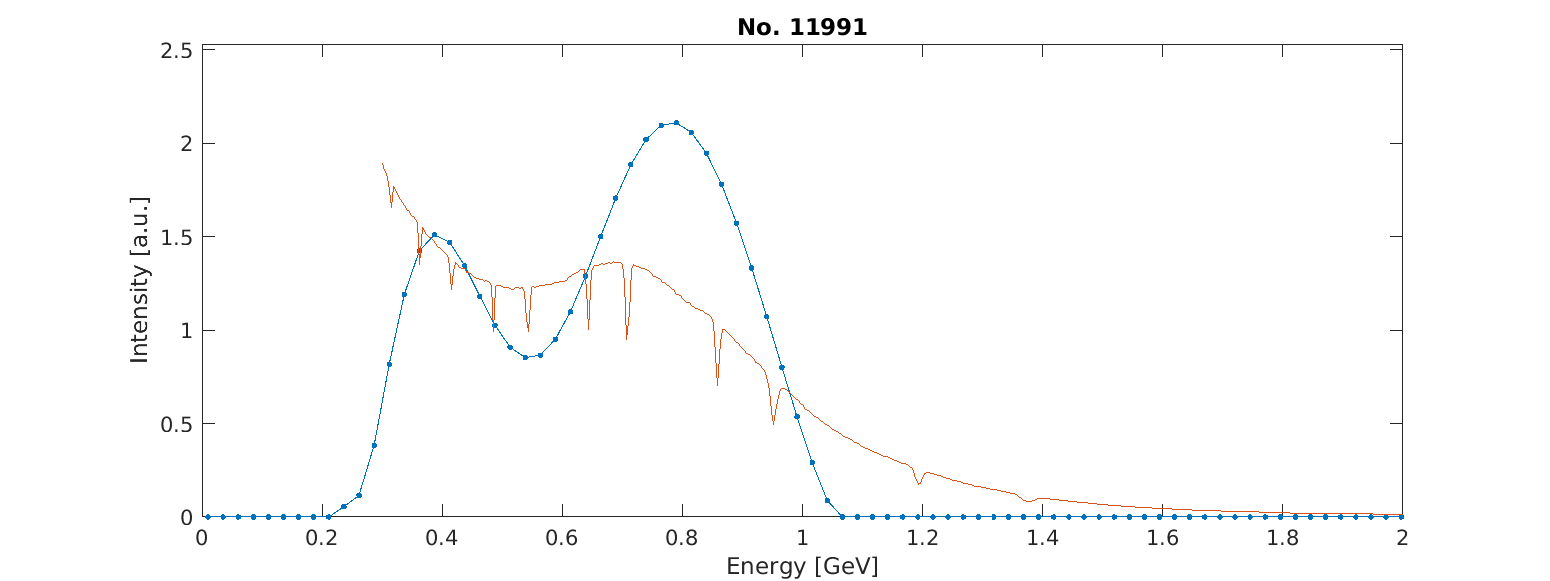
\includegraphics[width=9.0cm]{fig1a.png}
    \caption{\label{fig:fig1a.png}}
    \end{subfigure}
\quad
    \begin{subfigure}[b]{0.45\textwidth}
    \centering
    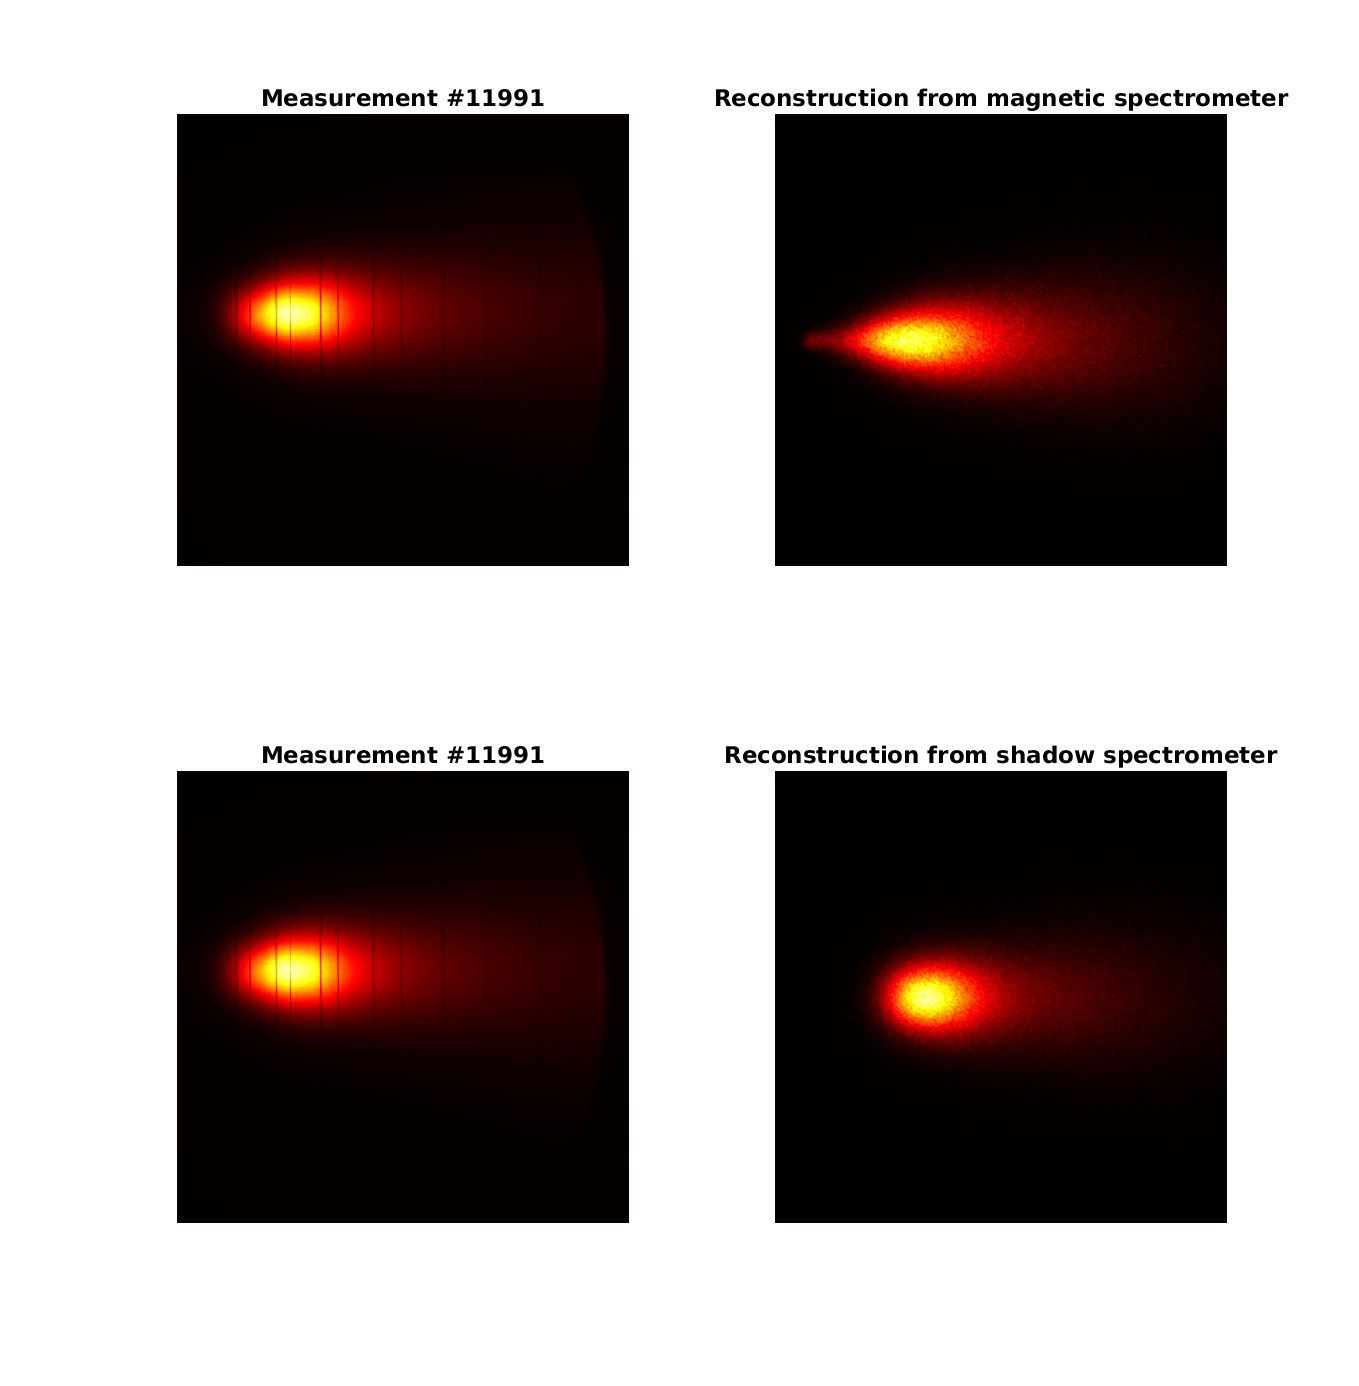
\includegraphics[width=9.0cm]{fig2_11991.png}
    \caption{\label{fig:fig2_11991.png}}
    \end{subfigure}


\captionsetup{justification=raggedright,singlelinecheck=false}
\caption{\label{fig:fig1a.png}}

\end{figure}



\section{No_12005}

\begin{figure}[b]

\centering

\quad
    \begin{subfigure}[b]{0.45\textwidth}
    \centering
    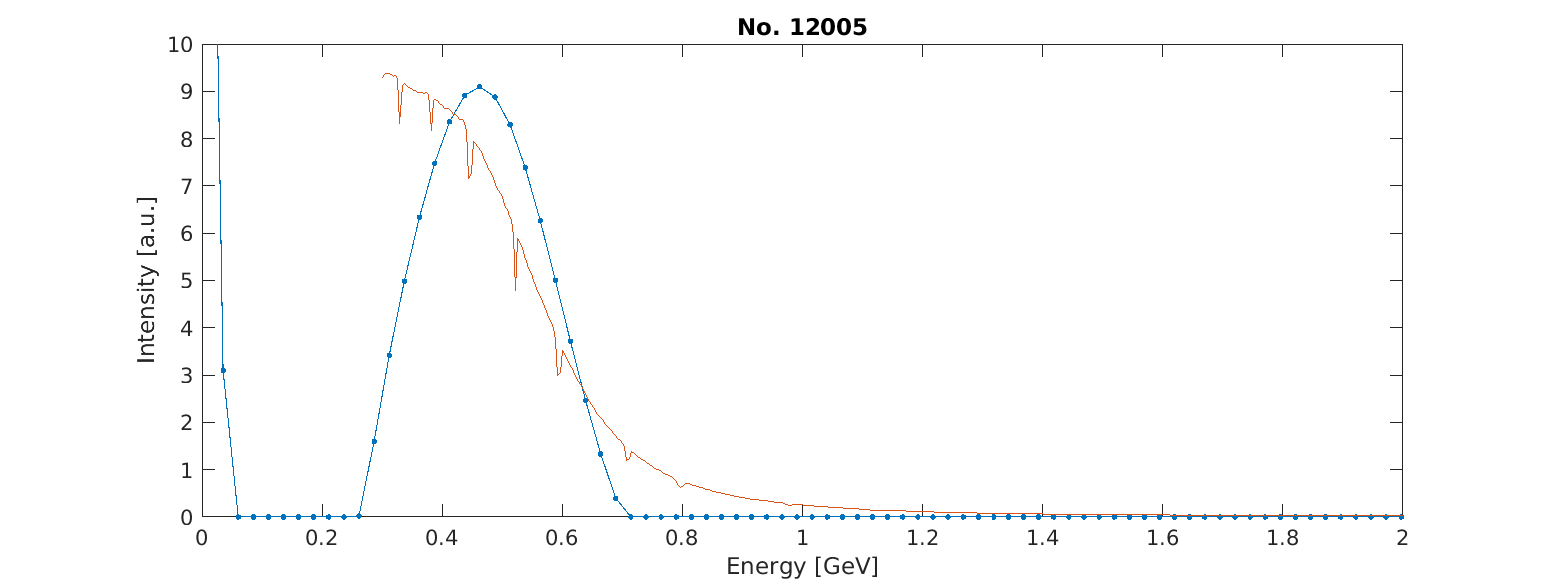
\includegraphics[width=9.0cm]{fig1k.png}
    \caption{\label{fig:fig1k.png}}
    \end{subfigure}
\quad
    \begin{subfigure}[b]{0.45\textwidth}
    \centering
    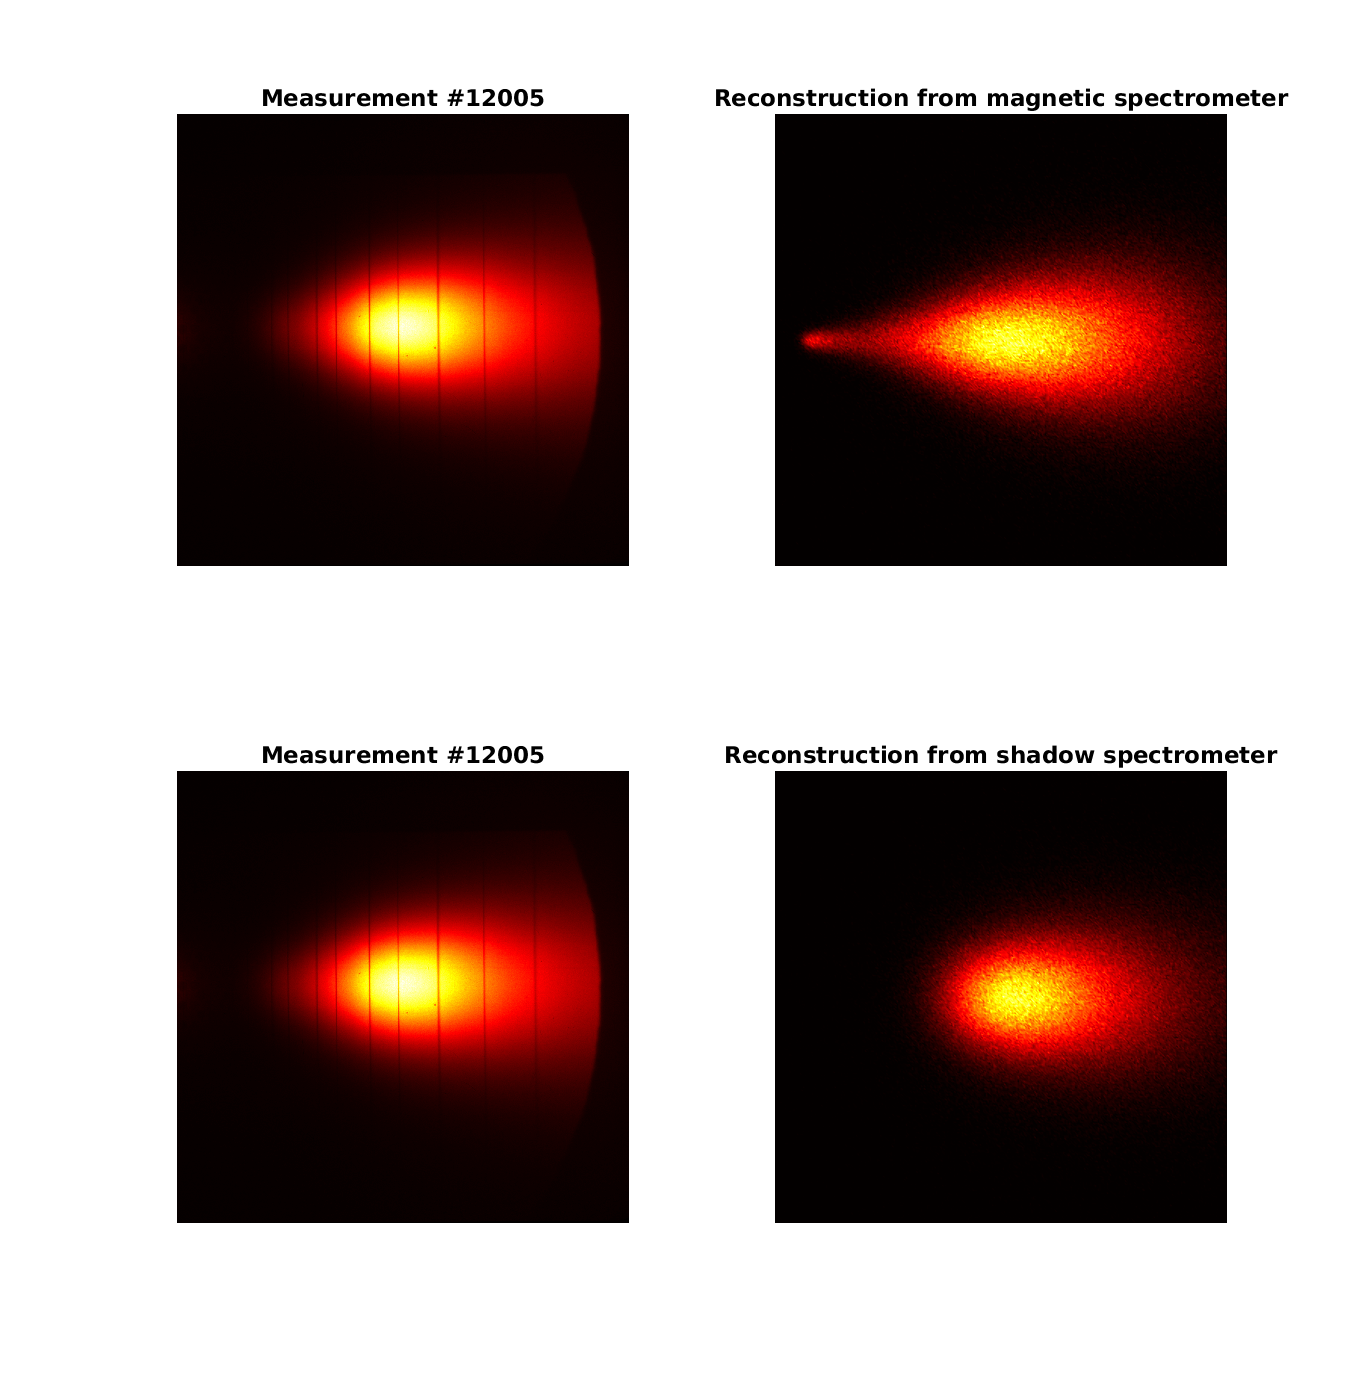
\includegraphics[width=9.0cm]{fig2_12005.png}
    \caption{\label{fig:fig2_12005.png}}
    \end{subfigure}


\captionsetup{justification=raggedright,singlelinecheck=false}
\caption{\label{fig:fig1k.png}}

\end{figure}



\section{No_12007}

\begin{figure}[b]

\centering

\quad
    \begin{subfigure}[b]{0.45\textwidth}
    \centering
    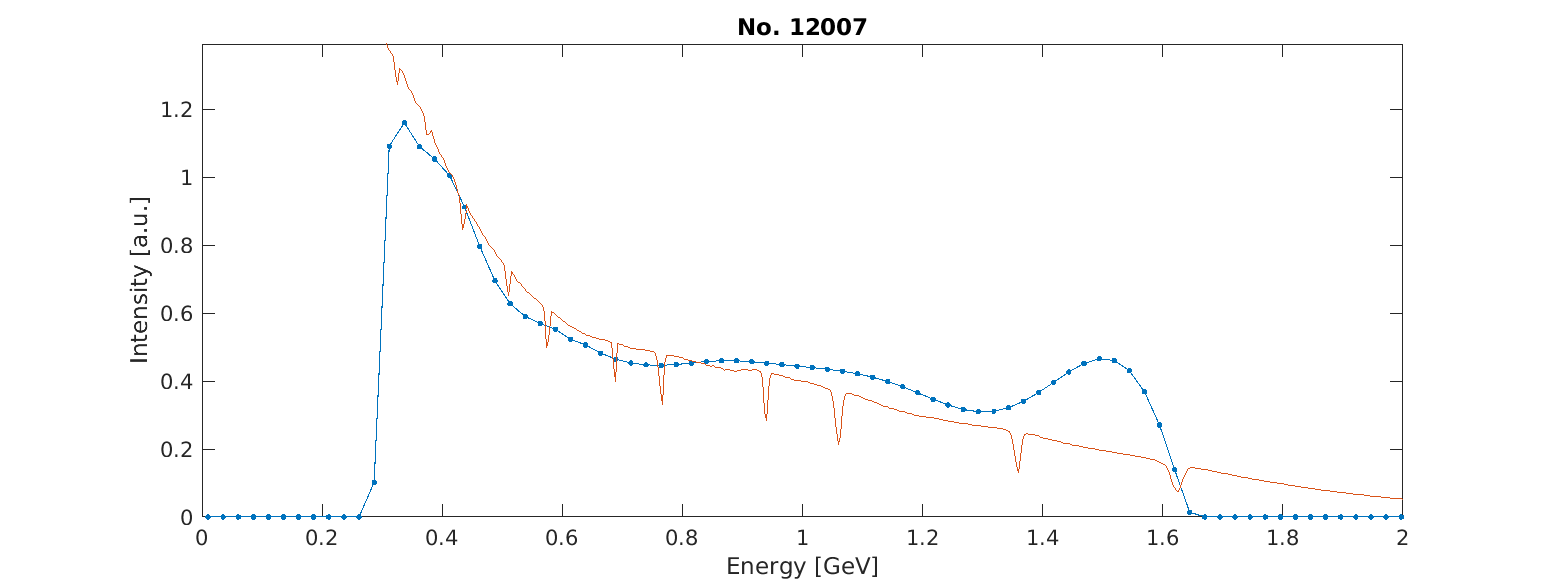
\includegraphics[width=9.0cm]{fig1j.png}
    \caption{\label{fig:fig1j.png}}
    \end{subfigure}
\quad
    \begin{subfigure}[b]{0.45\textwidth}
    \centering
    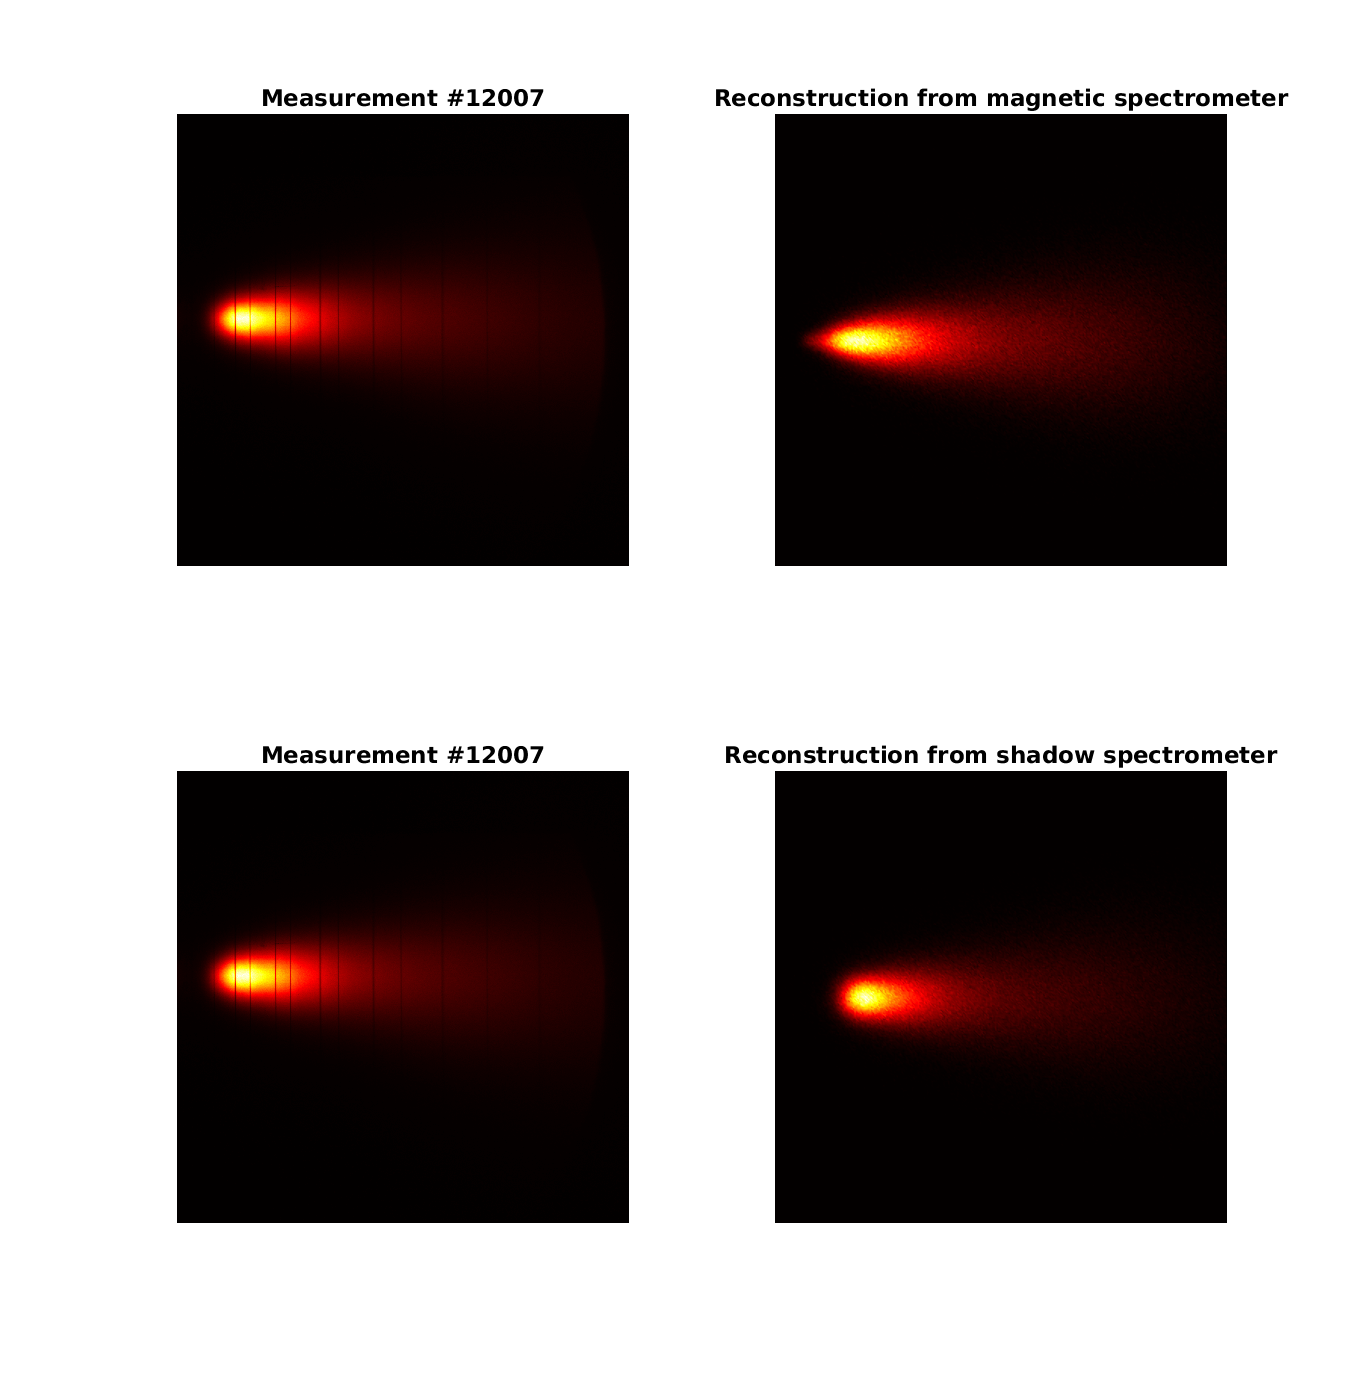
\includegraphics[width=9.0cm]{fig2_12007.png}
    \caption{\label{fig:fig2_12007.png}}
    \end{subfigure}


\captionsetup{justification=raggedright,singlelinecheck=false}
\caption{\label{fig:fig1j.png}}

\end{figure}



\section{No_12009}

\begin{figure}[b]

\centering

\quad
    \begin{subfigure}[b]{0.45\textwidth}
    \centering
    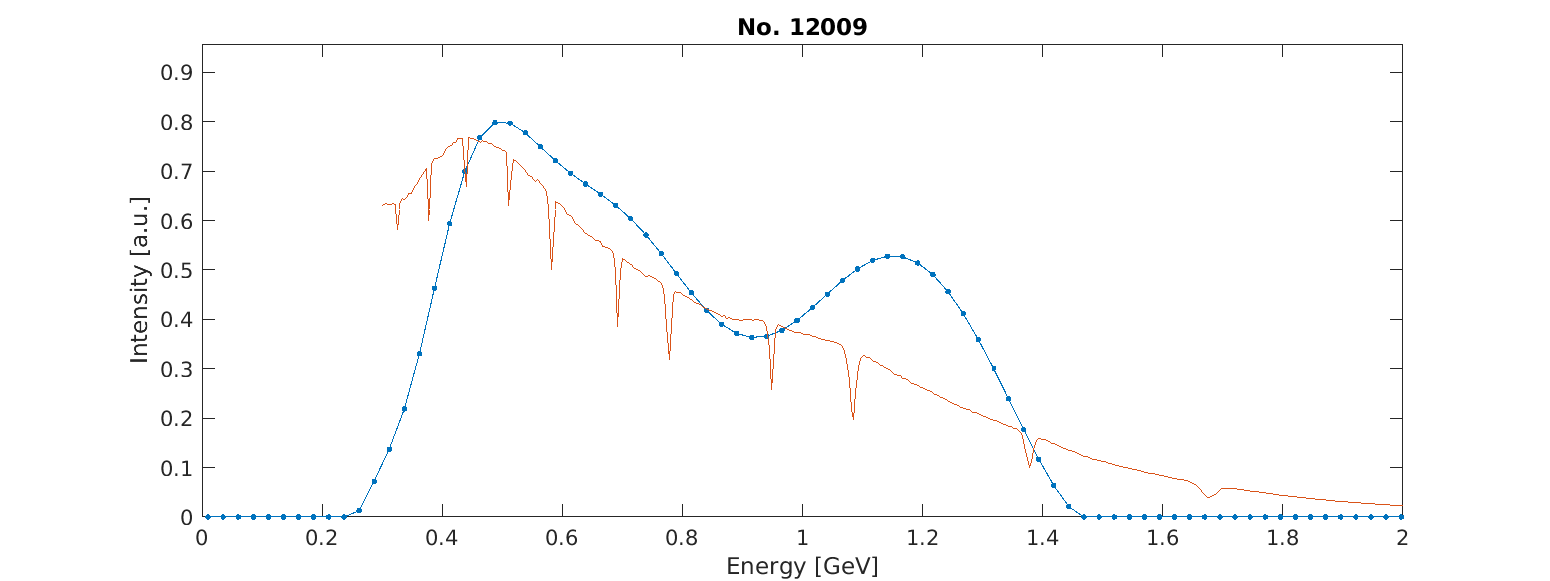
\includegraphics[width=9.0cm]{fig1i.png}
    \caption{\label{fig:fig1i.png}}
    \end{subfigure}
\quad
    \begin{subfigure}[b]{0.45\textwidth}
    \centering
    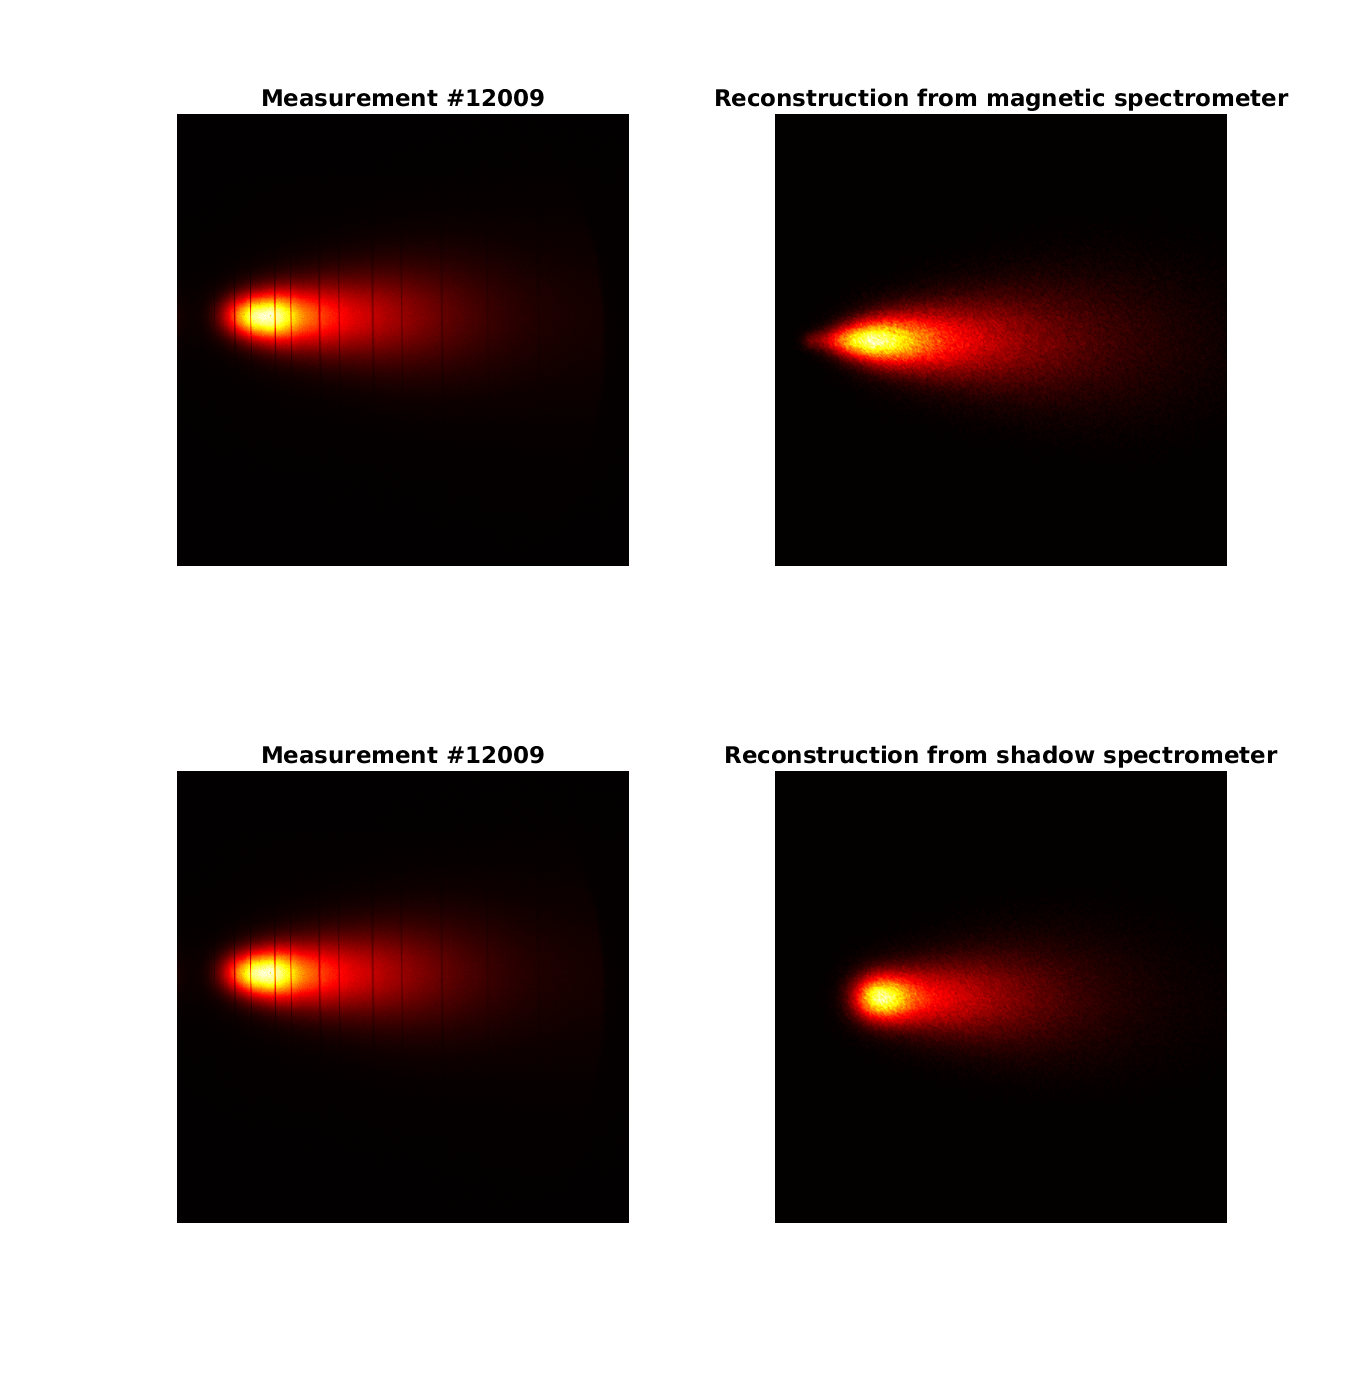
\includegraphics[width=9.0cm]{fig2_12009.png}
    \caption{\label{fig:fig2_12009.png}}
    \end{subfigure}


\captionsetup{justification=raggedright,singlelinecheck=false}
\caption{\label{fig:fig1i.png}}

\end{figure}



\section{No_12041}

\begin{figure}[b]

\centering

\quad
    \begin{subfigure}[b]{0.45\textwidth}
    \centering
    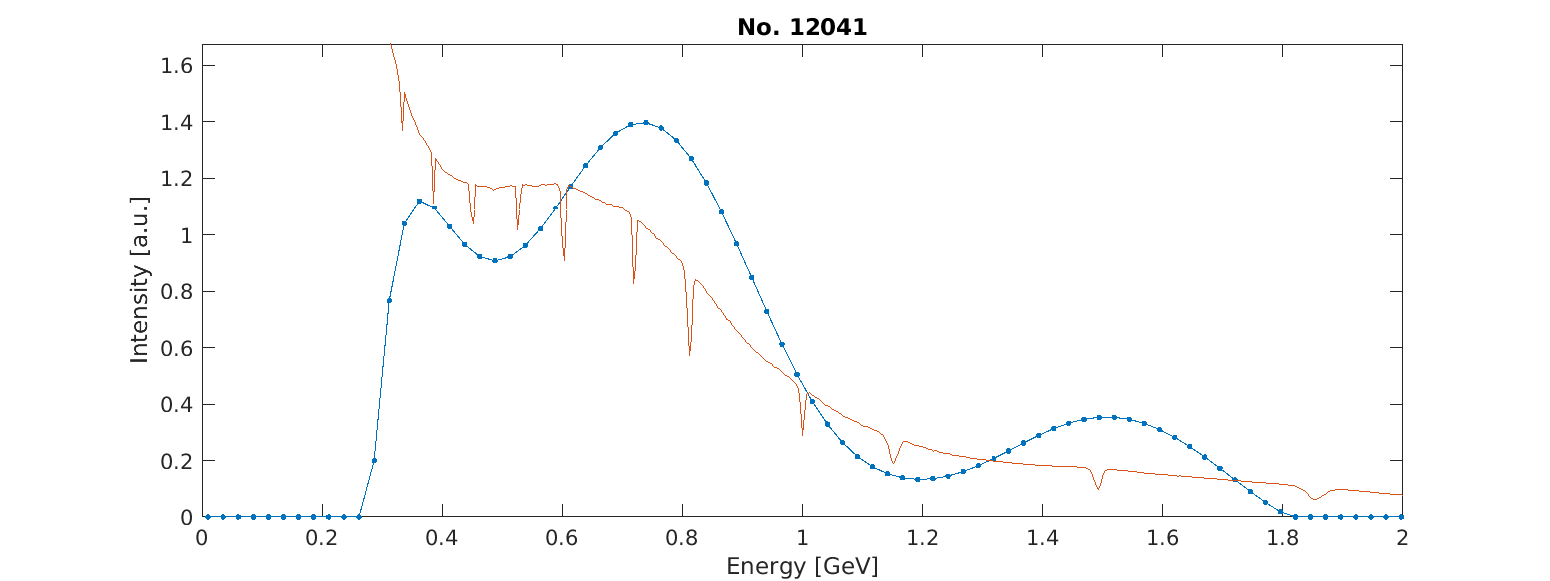
\includegraphics[width=9.0cm]{fig1h.png}
    \caption{\label{fig:fig1h.png}}
    \end{subfigure}
\quad
    \begin{subfigure}[b]{0.45\textwidth}
    \centering
    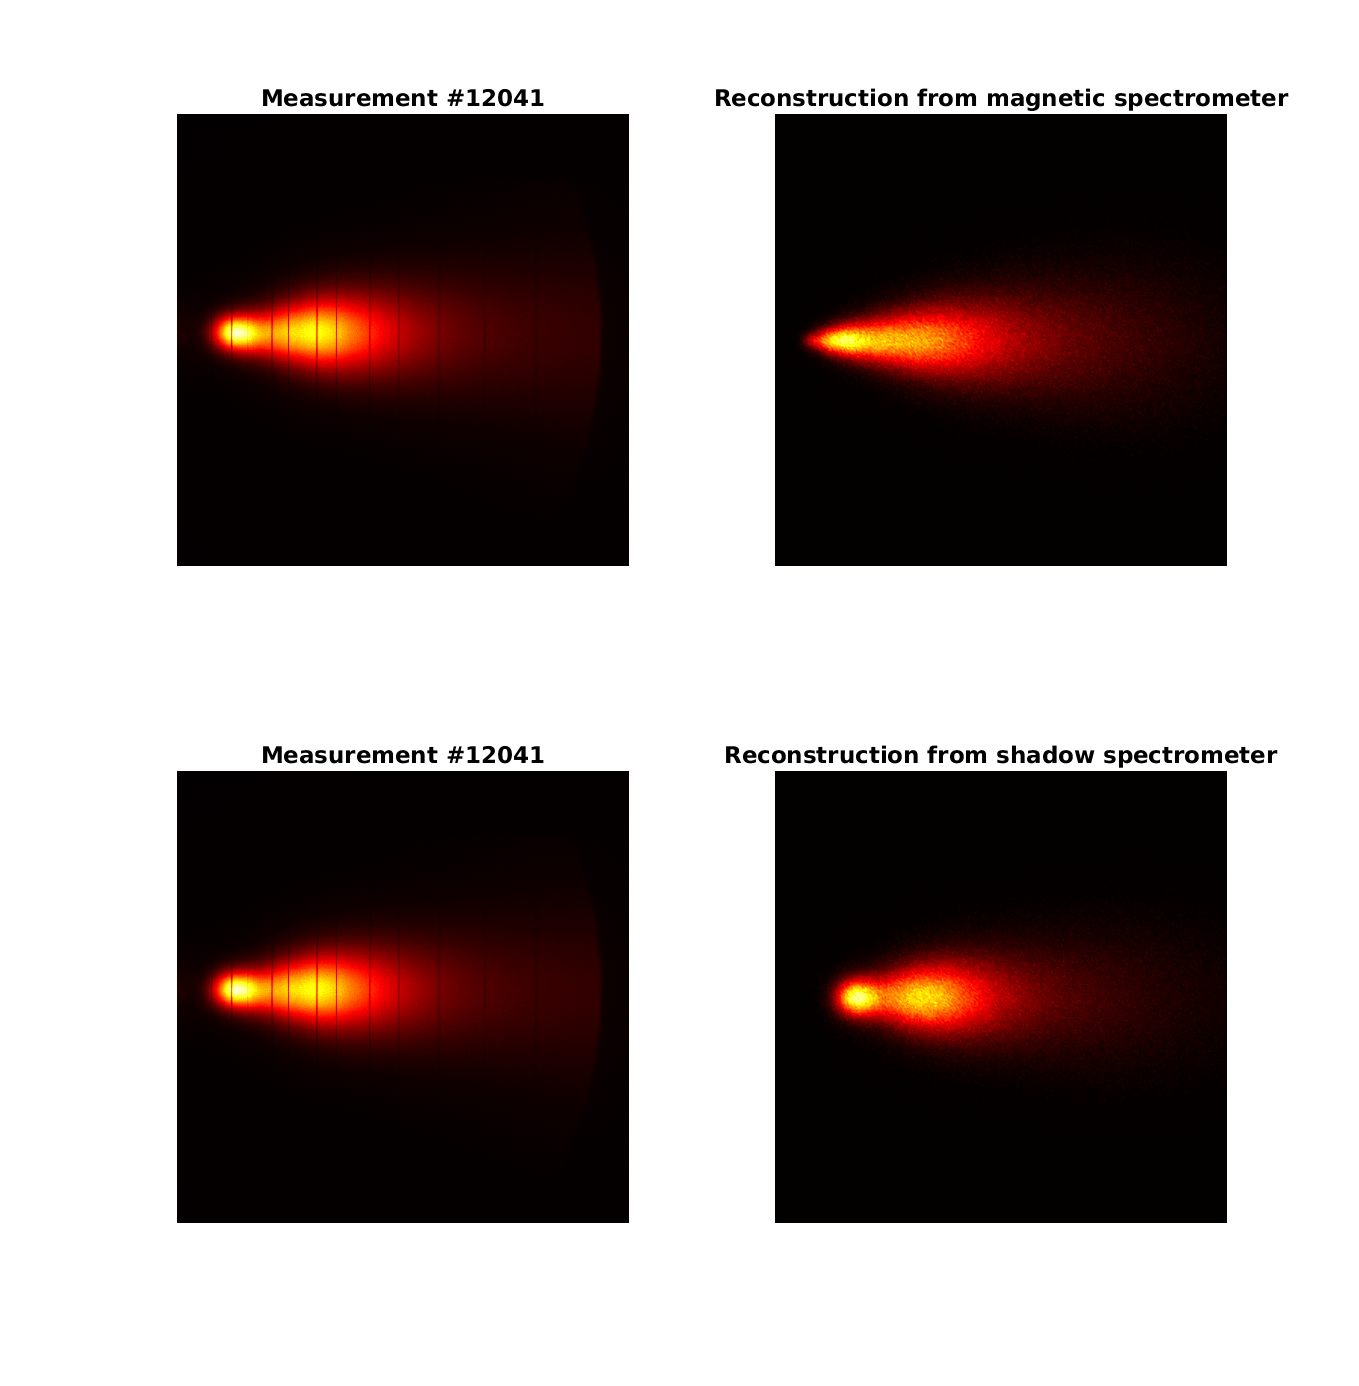
\includegraphics[width=9.0cm]{fig2_12041.png}
    \caption{\label{fig:fig2_12041.png}}
    \end{subfigure}


\captionsetup{justification=raggedright,singlelinecheck=false}
\caption{\label{fig:fig1h.png}}

\end{figure}



\section{No_12043}

\begin{figure}[b]

\centering

\quad
    \begin{subfigure}[b]{0.45\textwidth}
    \centering
    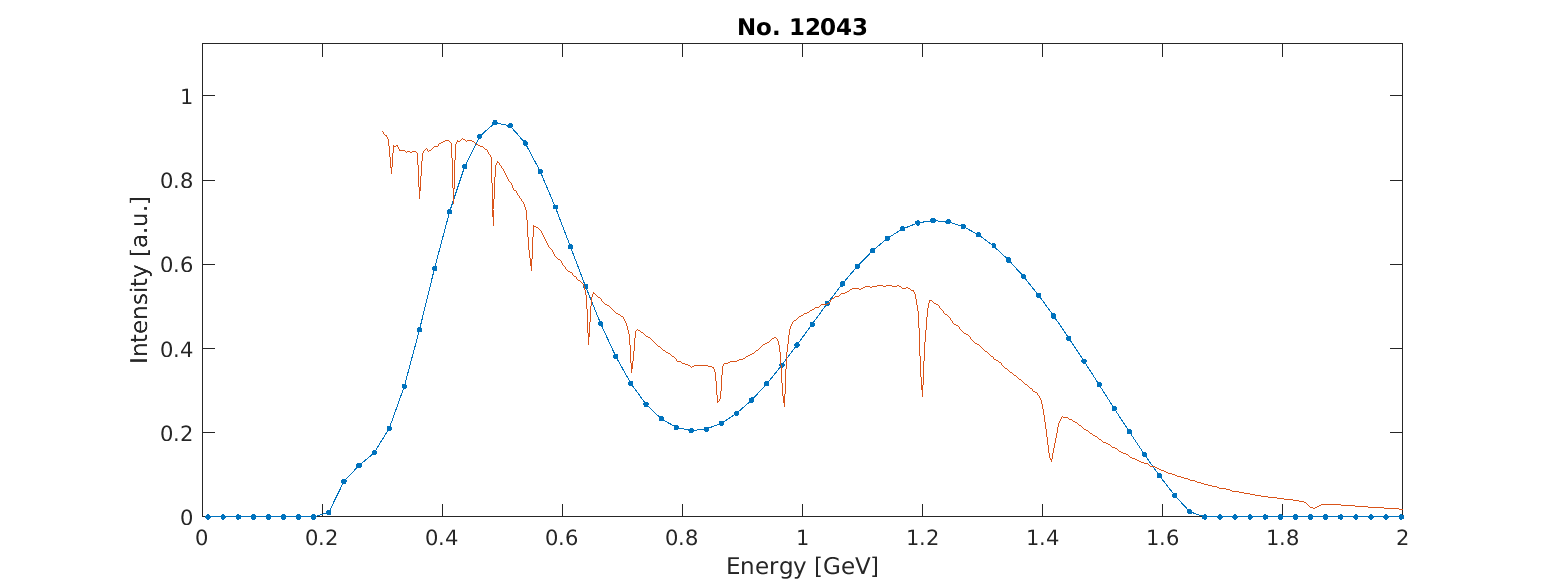
\includegraphics[width=9.0cm]{fig1g.png}
    \caption{\label{fig:fig1g.png}}
    \end{subfigure}
\quad
    \begin{subfigure}[b]{0.45\textwidth}
    \centering
    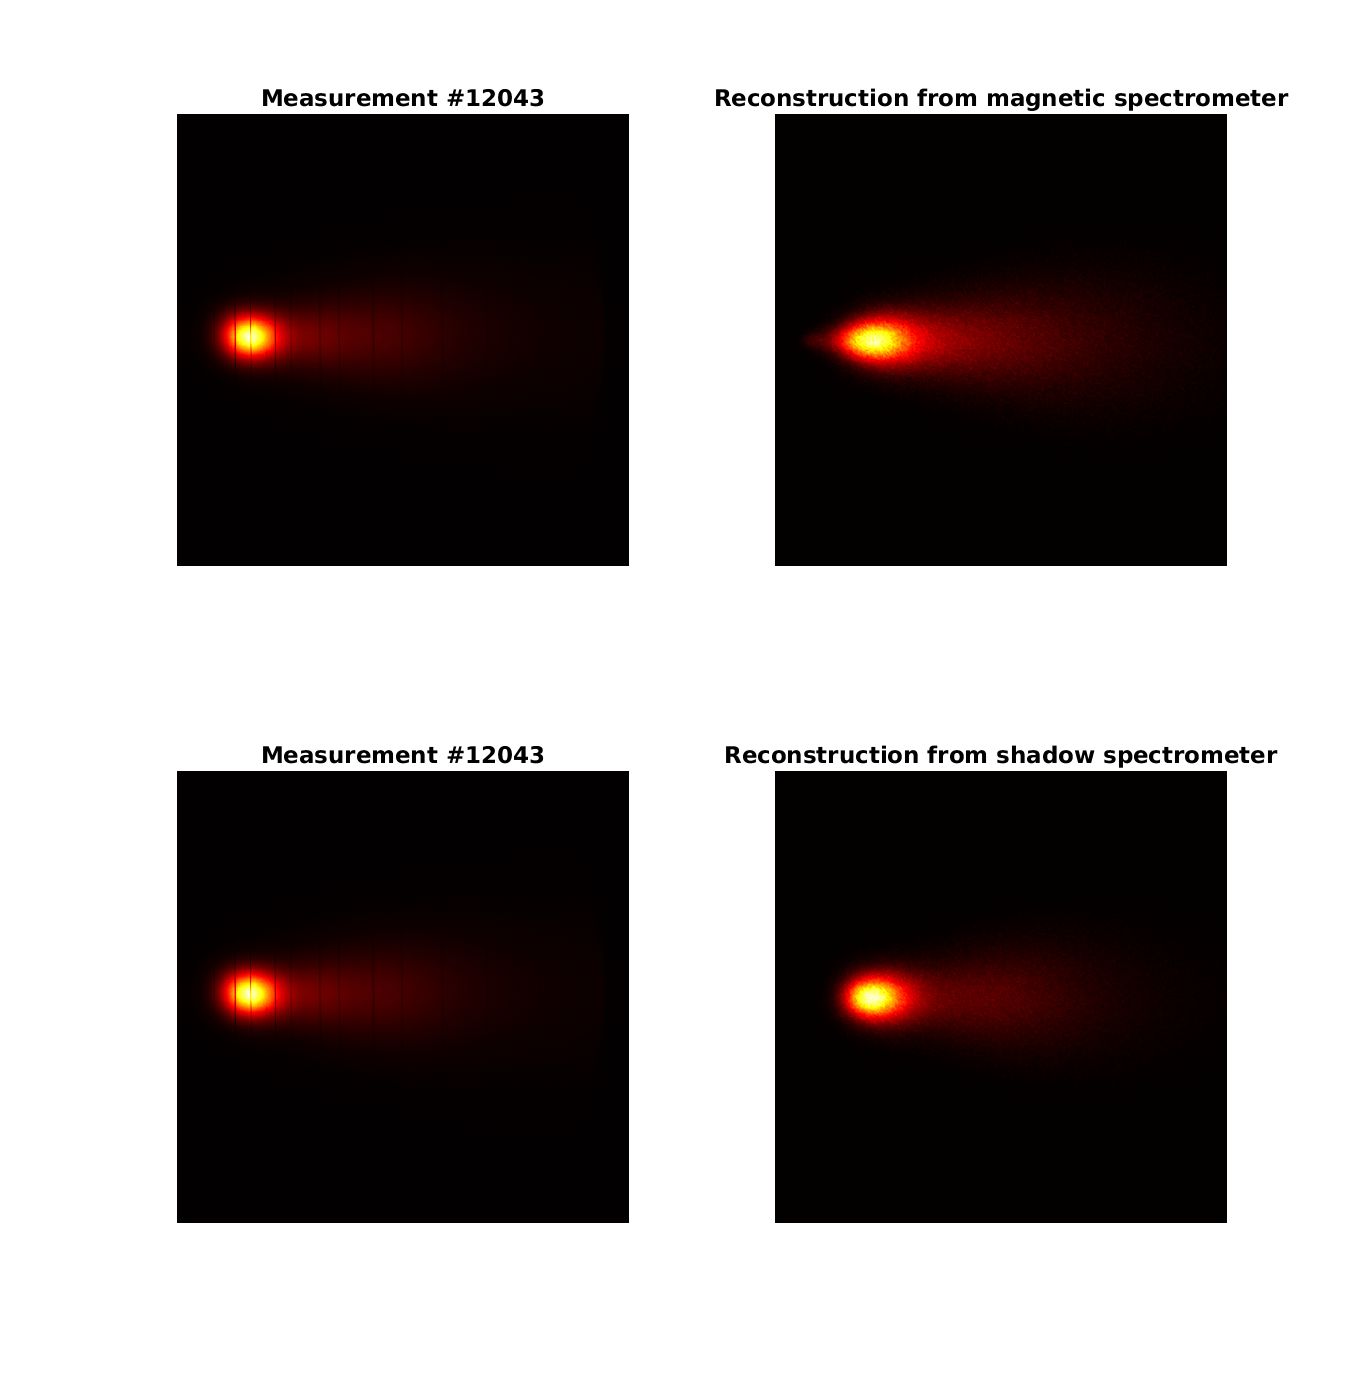
\includegraphics[width=9.0cm]{fig2_12043.png}
    \caption{\label{fig:fig2_12043.png}}
    \end{subfigure}


\captionsetup{justification=raggedright,singlelinecheck=false}
\caption{\label{fig:fig1g.png}}

\end{figure}



\section{No_12045}

\begin{figure}[b]

\centering

\quad
    \begin{subfigure}[b]{0.45\textwidth}
    \centering
    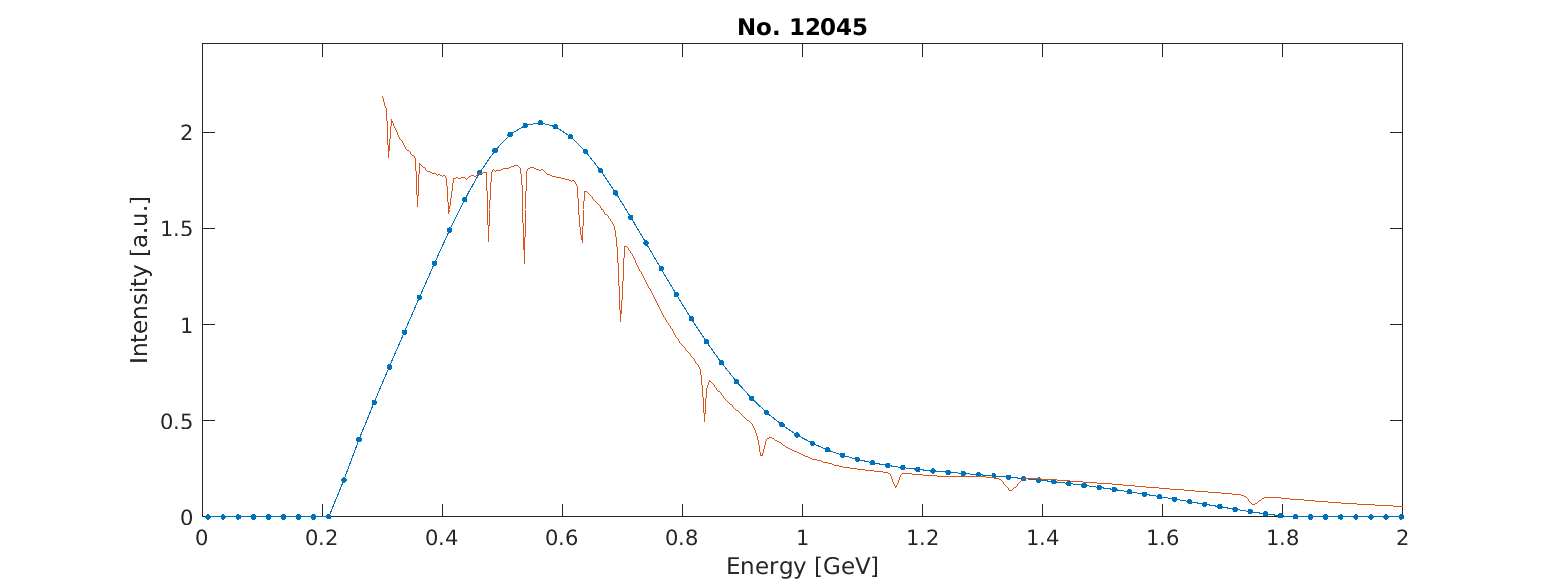
\includegraphics[width=9.0cm]{fig1f.png}
    \caption{\label{fig:fig1f.png}}
    \end{subfigure}
\quad
    \begin{subfigure}[b]{0.45\textwidth}
    \centering
    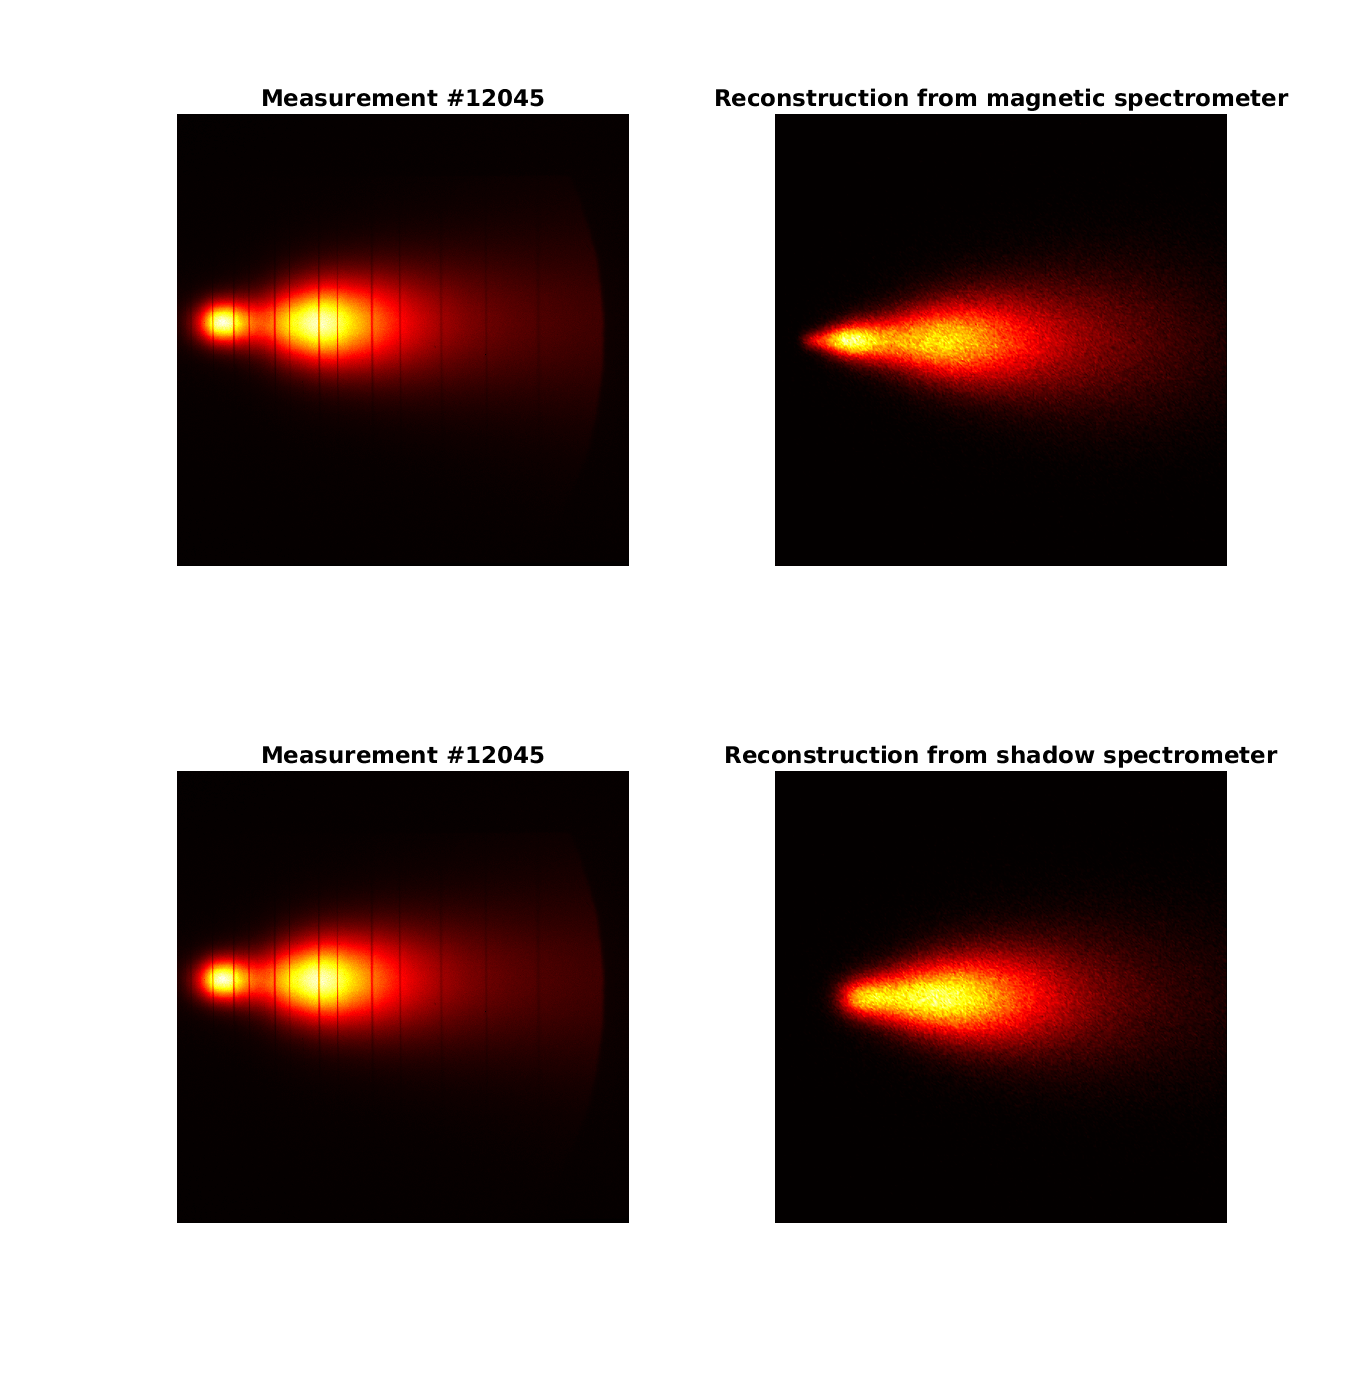
\includegraphics[width=9.0cm]{fig2_12045.png}
    \caption{\label{fig:fig2_12045.png}}
    \end{subfigure}


\captionsetup{justification=raggedright,singlelinecheck=false}
\caption{\label{fig:fig1f.png}}

\end{figure}



\section{No_12047}

\begin{figure}[b]

\centering

\quad
    \begin{subfigure}[b]{0.45\textwidth}
    \centering
    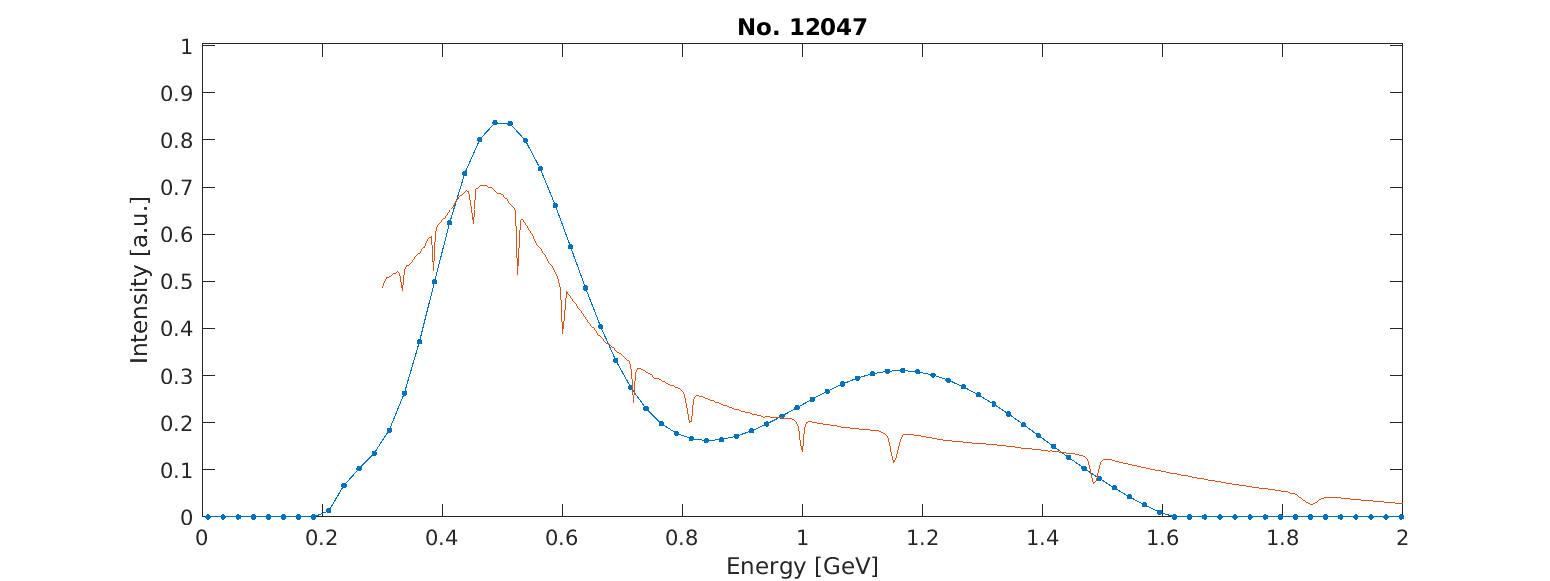
\includegraphics[width=9.0cm]{fig1e.png}
    \caption{\label{fig:fig1e.png}}
    \end{subfigure}
\quad
    \begin{subfigure}[b]{0.45\textwidth}
    \centering
    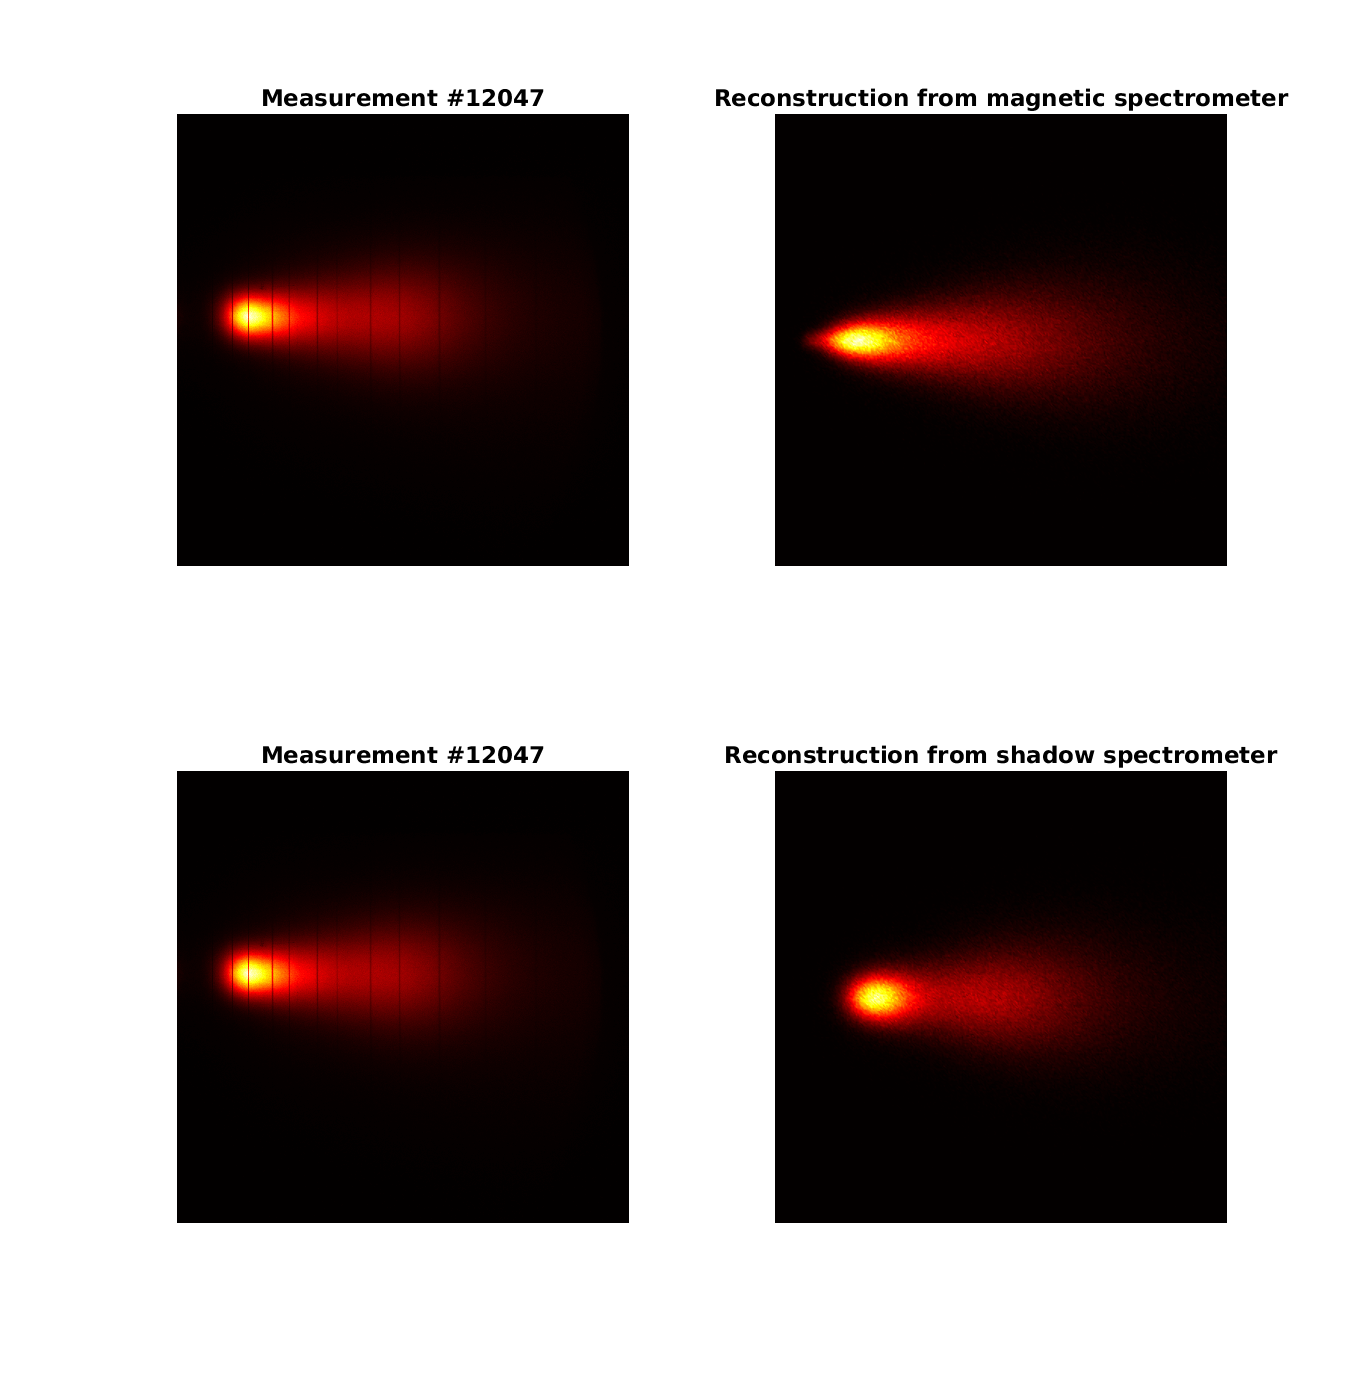
\includegraphics[width=9.0cm]{fig2_12047.png}
    \caption{\label{fig:fig2_12047.png}}
    \end{subfigure}


\captionsetup{justification=raggedright,singlelinecheck=false}
\caption{\label{fig:fig1e.png}}

\end{figure}



\section{No_12049}

\begin{figure}[b]

\centering

\quad
    \begin{subfigure}[b]{0.45\textwidth}
    \centering
    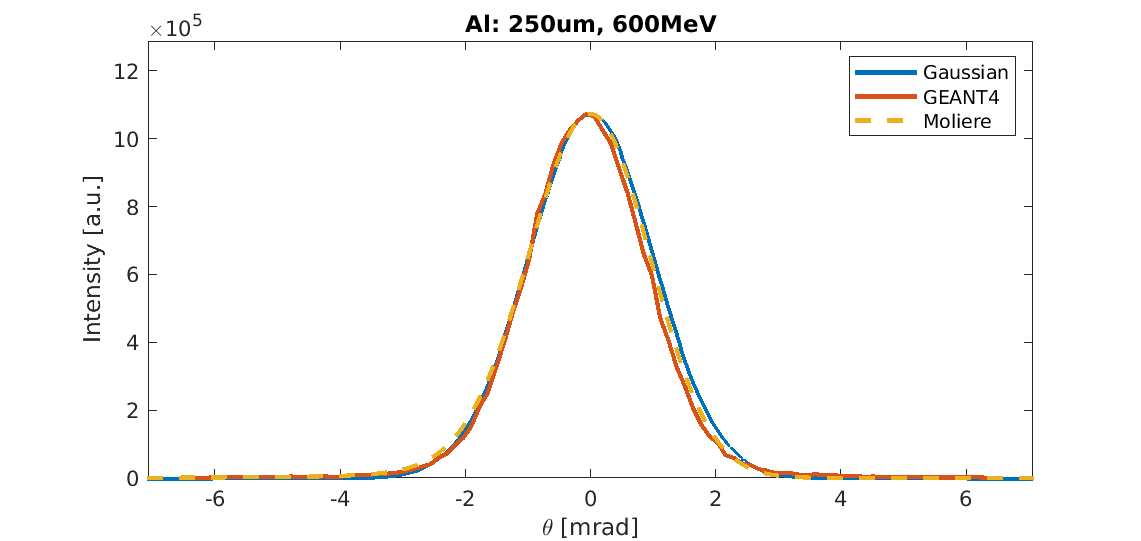
\includegraphics[width=9.0cm]{fig1d.png}
    \caption{\label{fig:fig1d.png}}
    \end{subfigure}
\quad
    \begin{subfigure}[b]{0.45\textwidth}
    \centering
    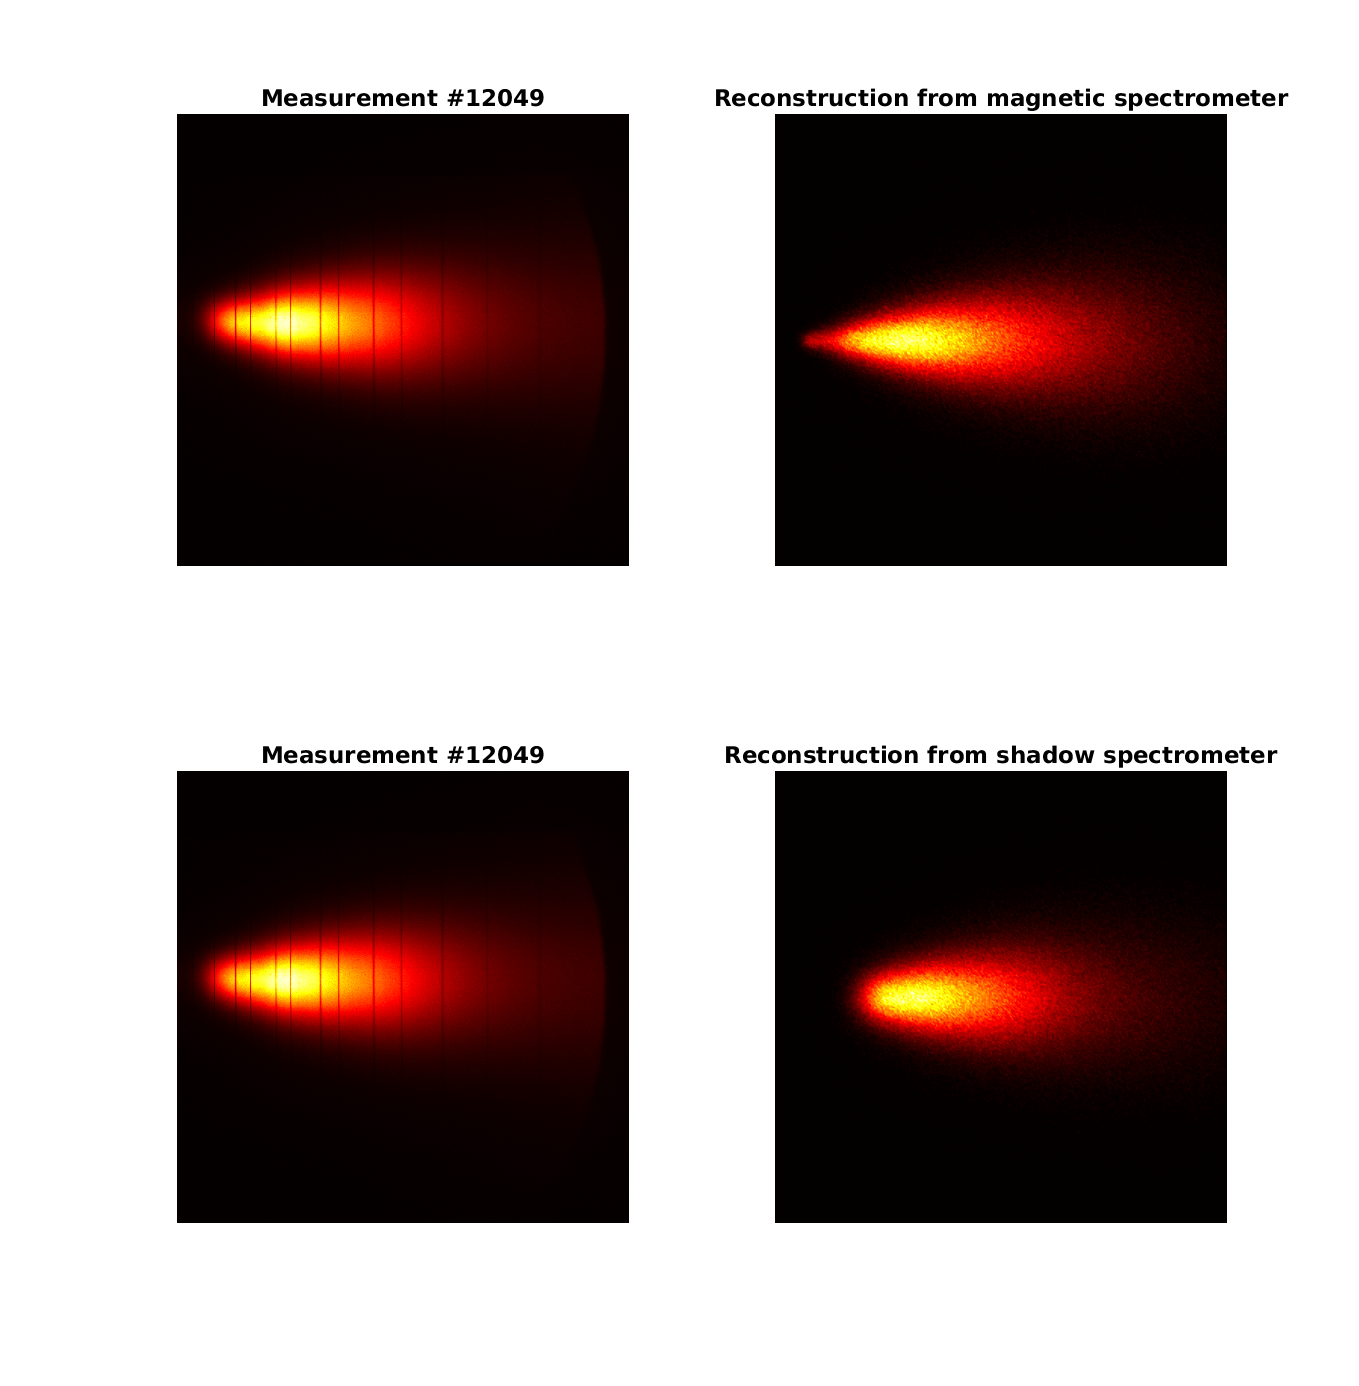
\includegraphics[width=9.0cm]{fig2_12049.png}
    \caption{\label{fig:fig2_12049.png}}
    \end{subfigure}


\captionsetup{justification=raggedright,singlelinecheck=false}
\caption{\label{fig:fig1d.png}}

\end{figure}



\section{No_12053}

\begin{figure}[b]

\centering

\quad
    \begin{subfigure}[b]{0.45\textwidth}
    \centering
    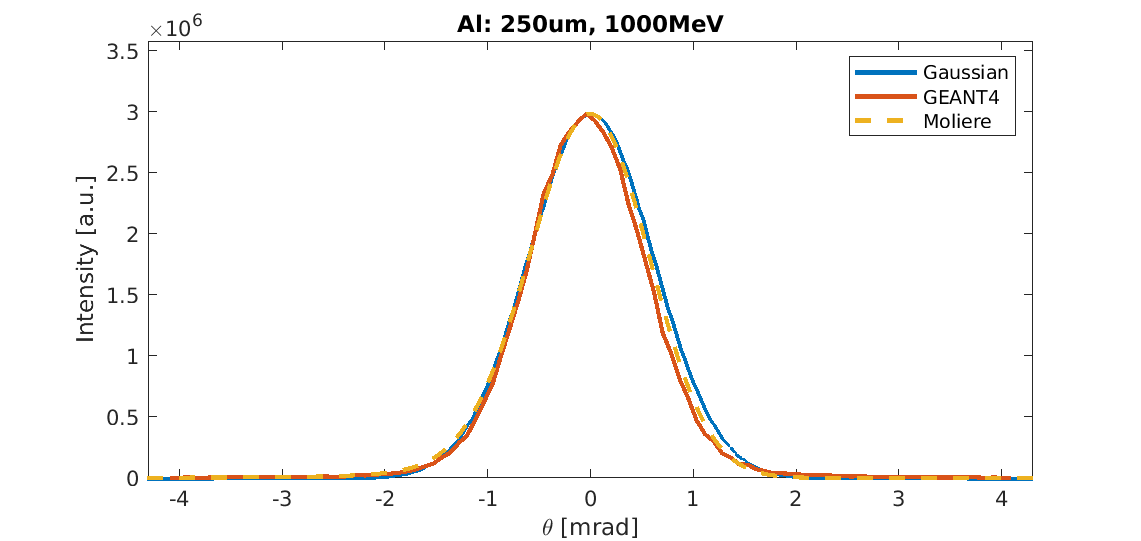
\includegraphics[width=9.0cm]{fig1c.png}
    \caption{\label{fig:fig1c.png}}
    \end{subfigure}
\quad
    \begin{subfigure}[b]{0.45\textwidth}
    \centering
    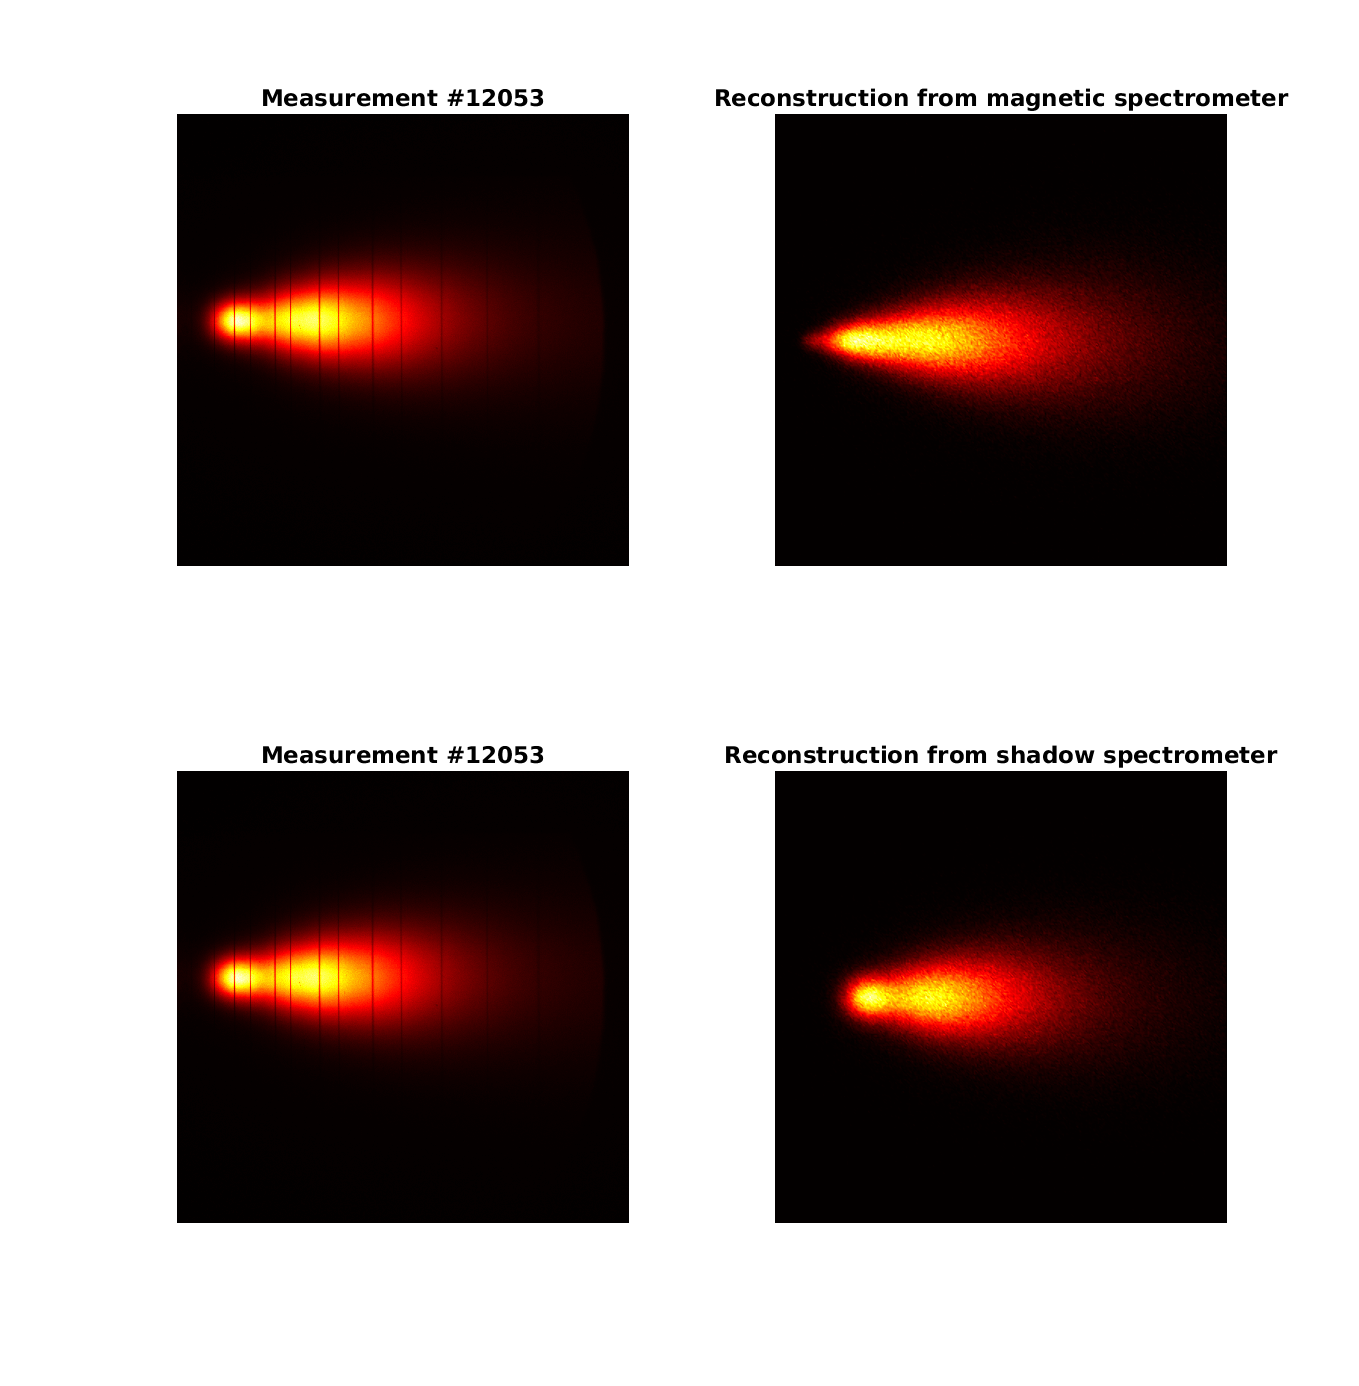
\includegraphics[width=9.0cm]{fig2_12053.png}
    \caption{\label{fig:fig2_12053.png}}
    \end{subfigure}


\captionsetup{justification=raggedright,singlelinecheck=false}
\caption{\label{fig:fig1c.png}}

\end{figure}



\section{No_12045}

\begin{figure}[b]

\centering

\quad
    \begin{subfigure}[b]{0.45\textwidth}
    \centering
    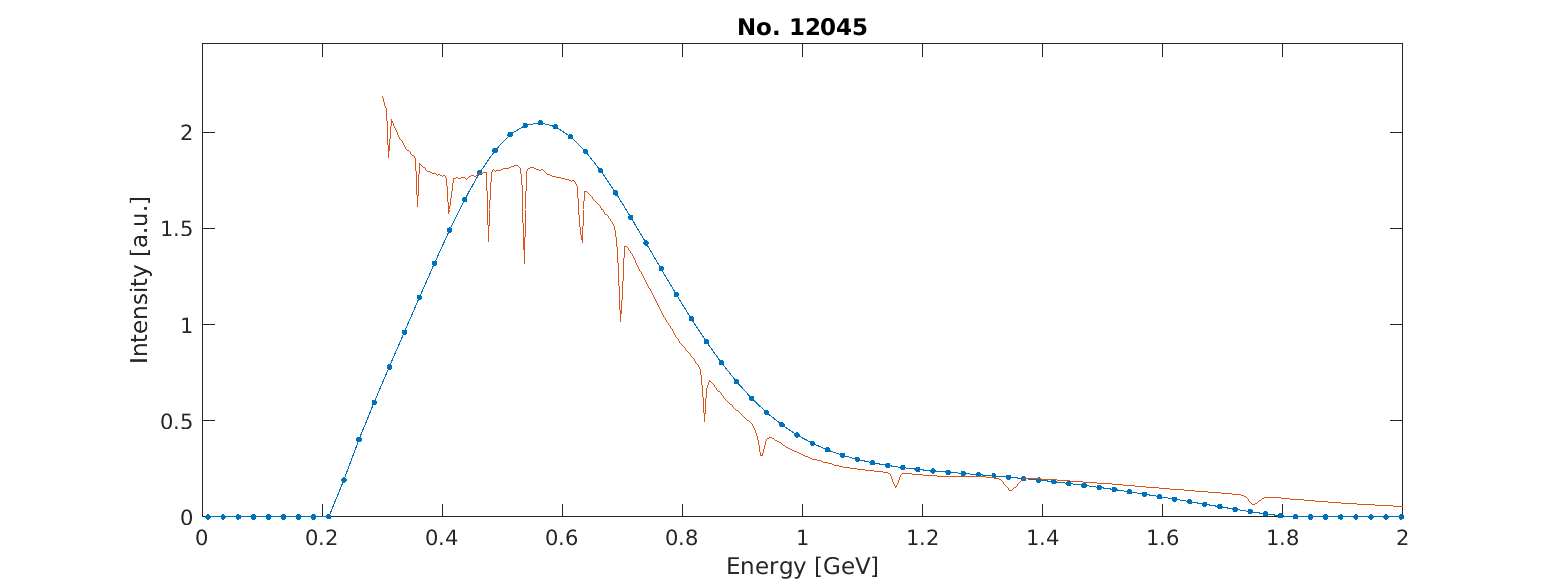
\includegraphics[width=9.0cm]{fig1f.png}
    \caption{\label{fig:fig1f.png}}
    \end{subfigure}
\quad
    \begin{subfigure}[b]{0.45\textwidth}
    \centering
    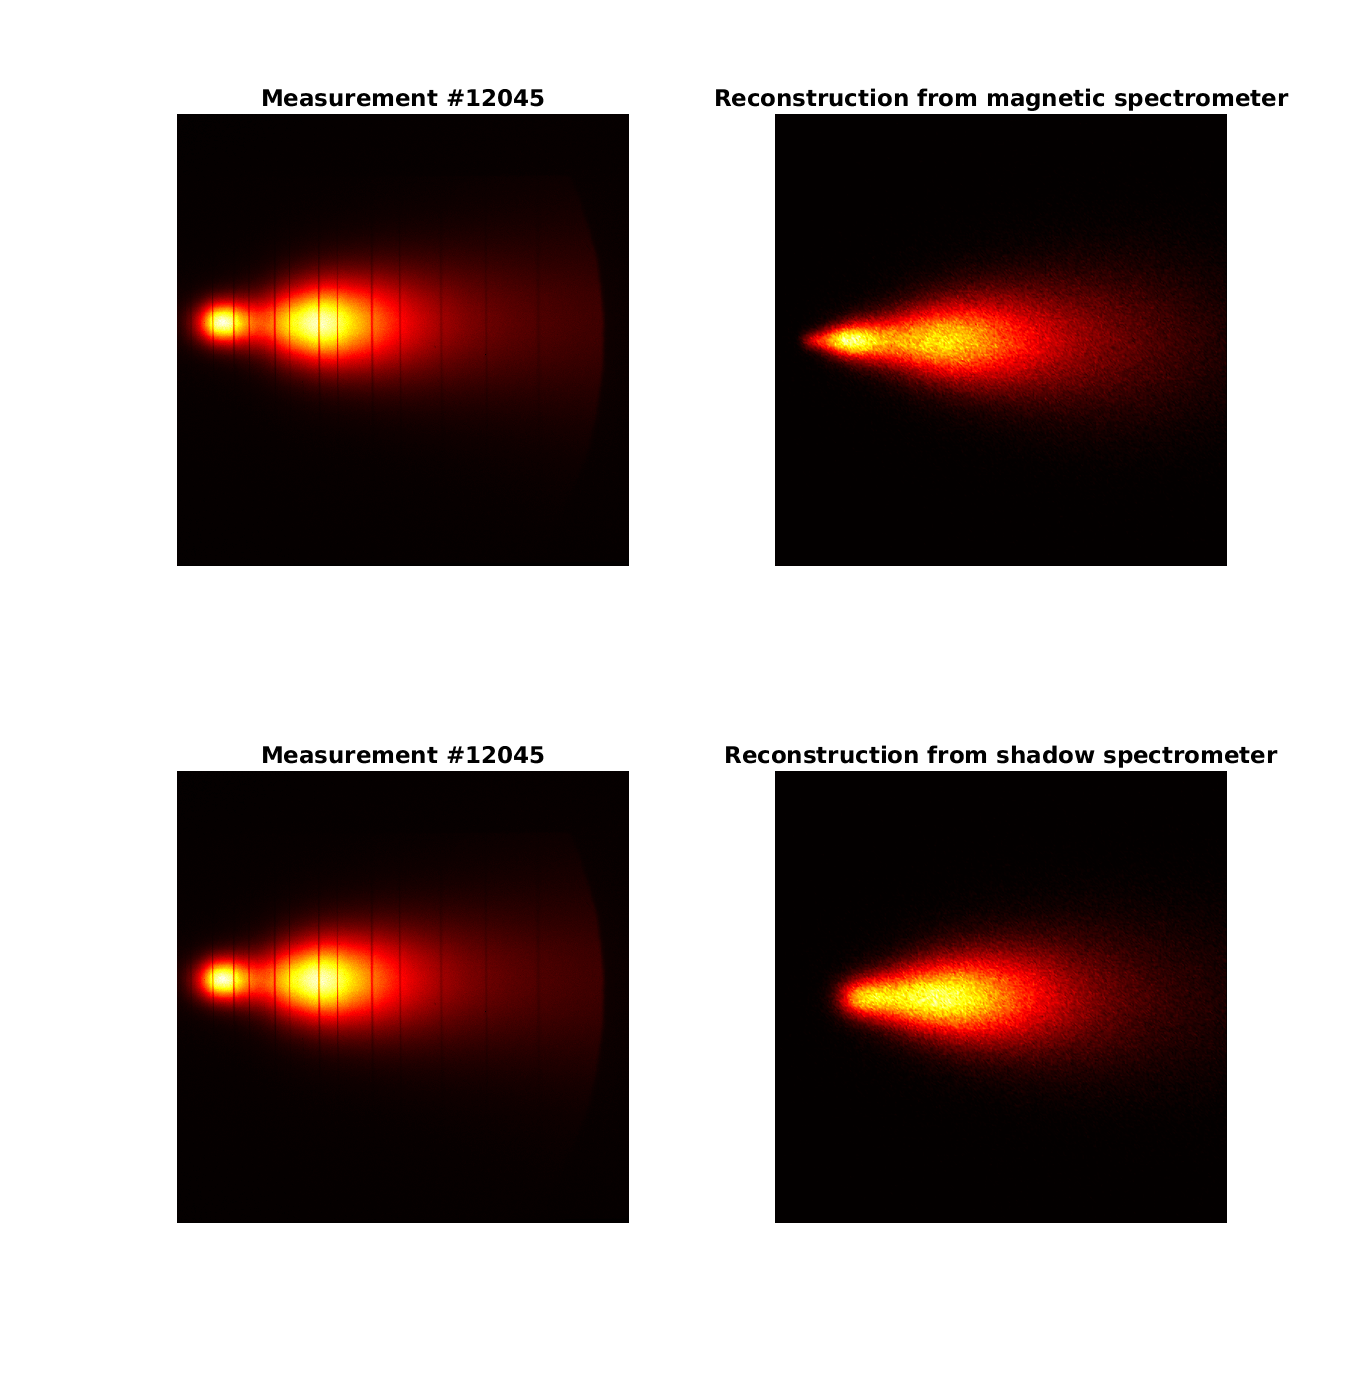
\includegraphics[width=9.0cm]{fig2_12045.png}
    \caption{\label{fig:fig2_12045.png}}
    \end{subfigure}


\captionsetup{justification=raggedright,singlelinecheck=false}
\caption{\label{fig:fig1f.png}}

\end{figure}



\section{No_12057}

\begin{figure}[b]

\centering

\quad
    \begin{subfigure}[b]{0.45\textwidth}
    \centering
    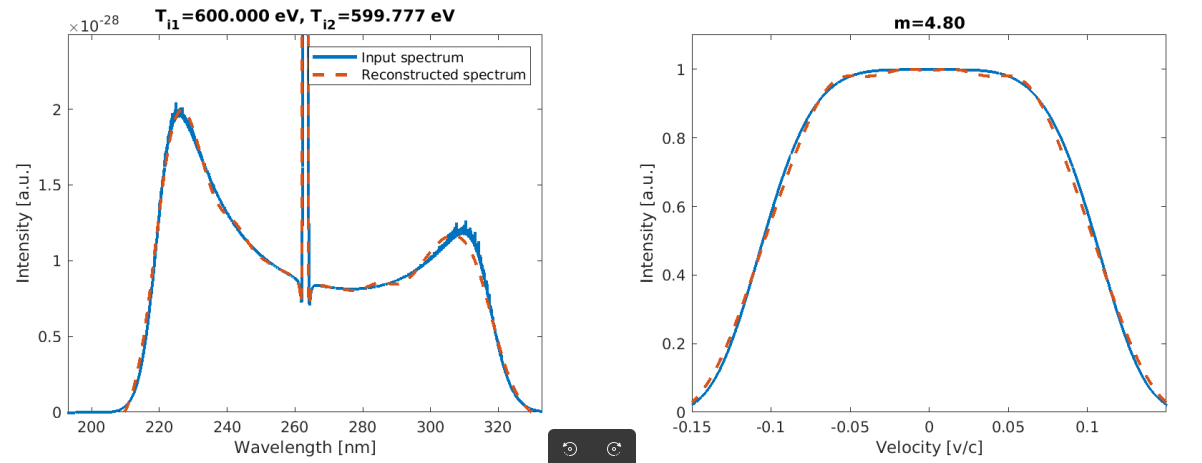
\includegraphics[width=9.0cm]{fig1b.png}
    \caption{\label{fig:fig1b.png}}
    \end{subfigure}
\quad
    \begin{subfigure}[b]{0.45\textwidth}
    \centering
    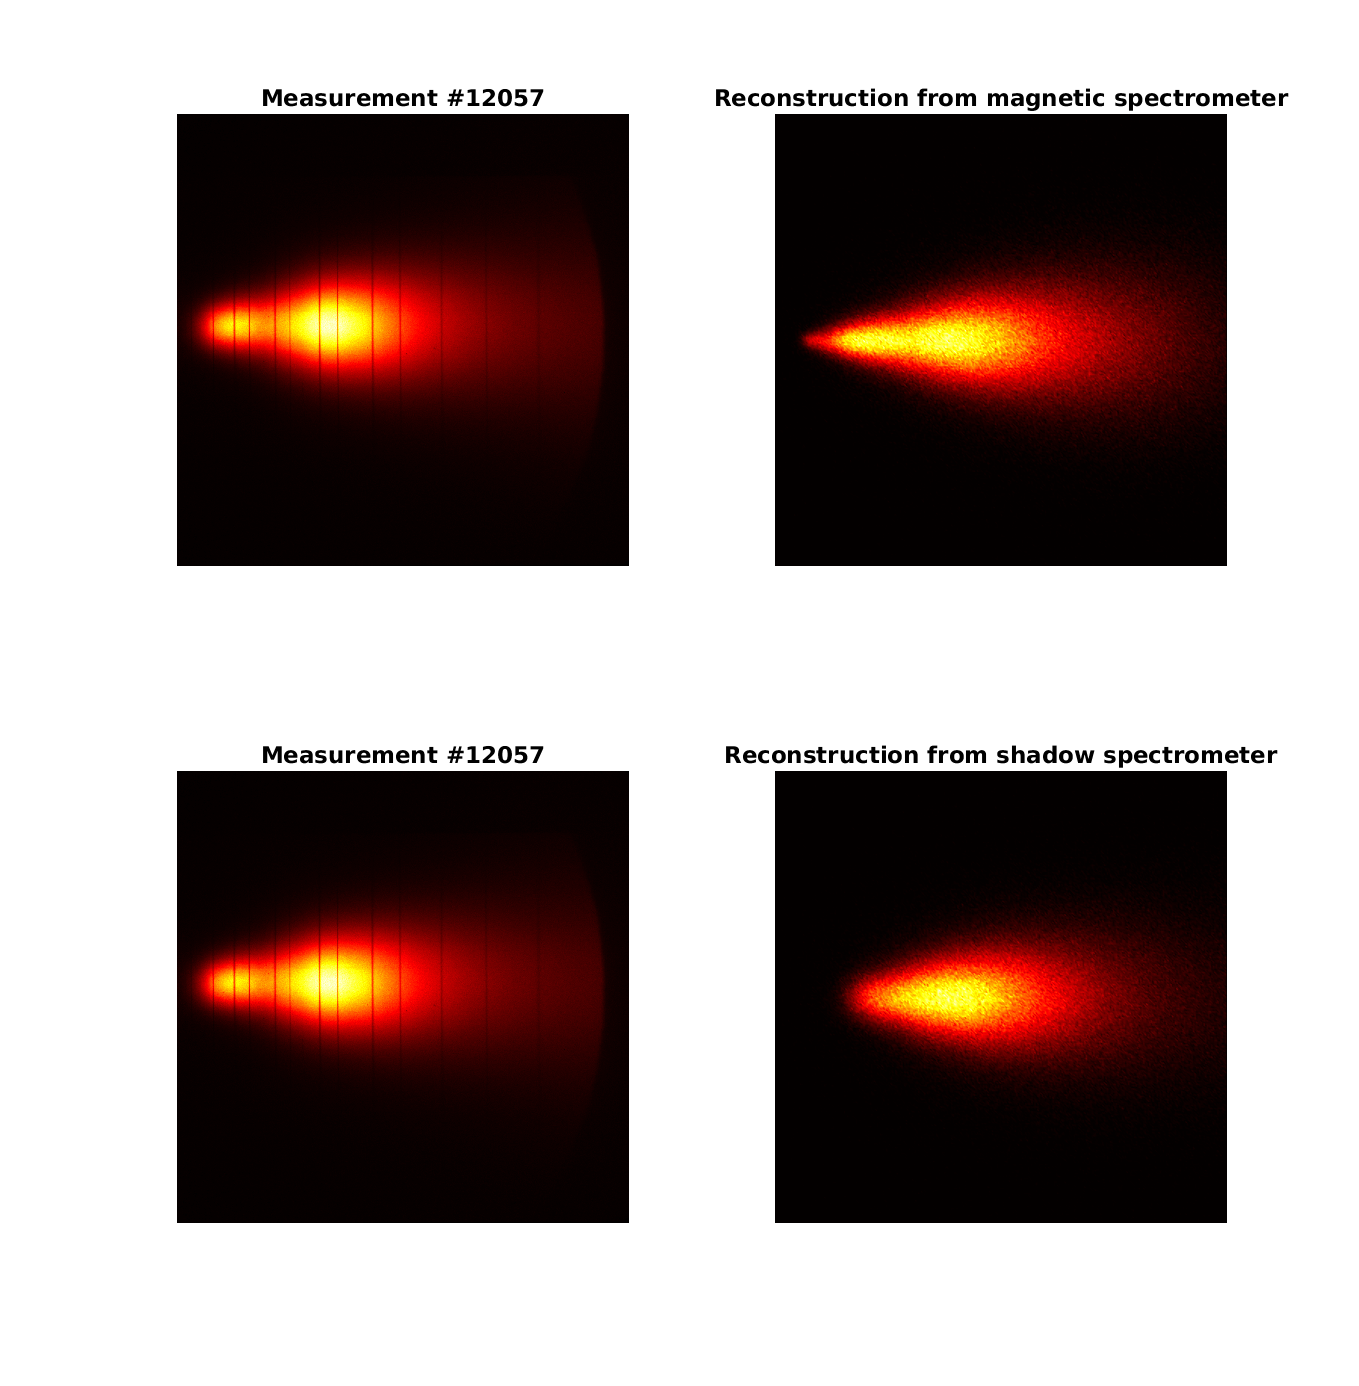
\includegraphics[width=9.0cm]{fig2_12057.png}
    \caption{\label{fig:fig2_12057.png}}
    \end{subfigure}


\captionsetup{justification=raggedright,singlelinecheck=false}
\caption{\label{fig:fig1b.png}}

\end{figure}






\nocite{*}

\bibliography{apssamp1}

\begin{filecontents}{apssamp1.bib}

\end{filecontents}

\end{document}
%
% ****** End of file apssamp.tex ******






